\section{ПРИЛОЖЕНИЕ Б} \label{ПРИЛОЖЕНИЕ Б}
\addcontentsline{toc}{section}{ПРИЛОЖЕНИЕ Б}
\\
\newline
\newline
\newline
\begin{figure}[ht!]
	\centering{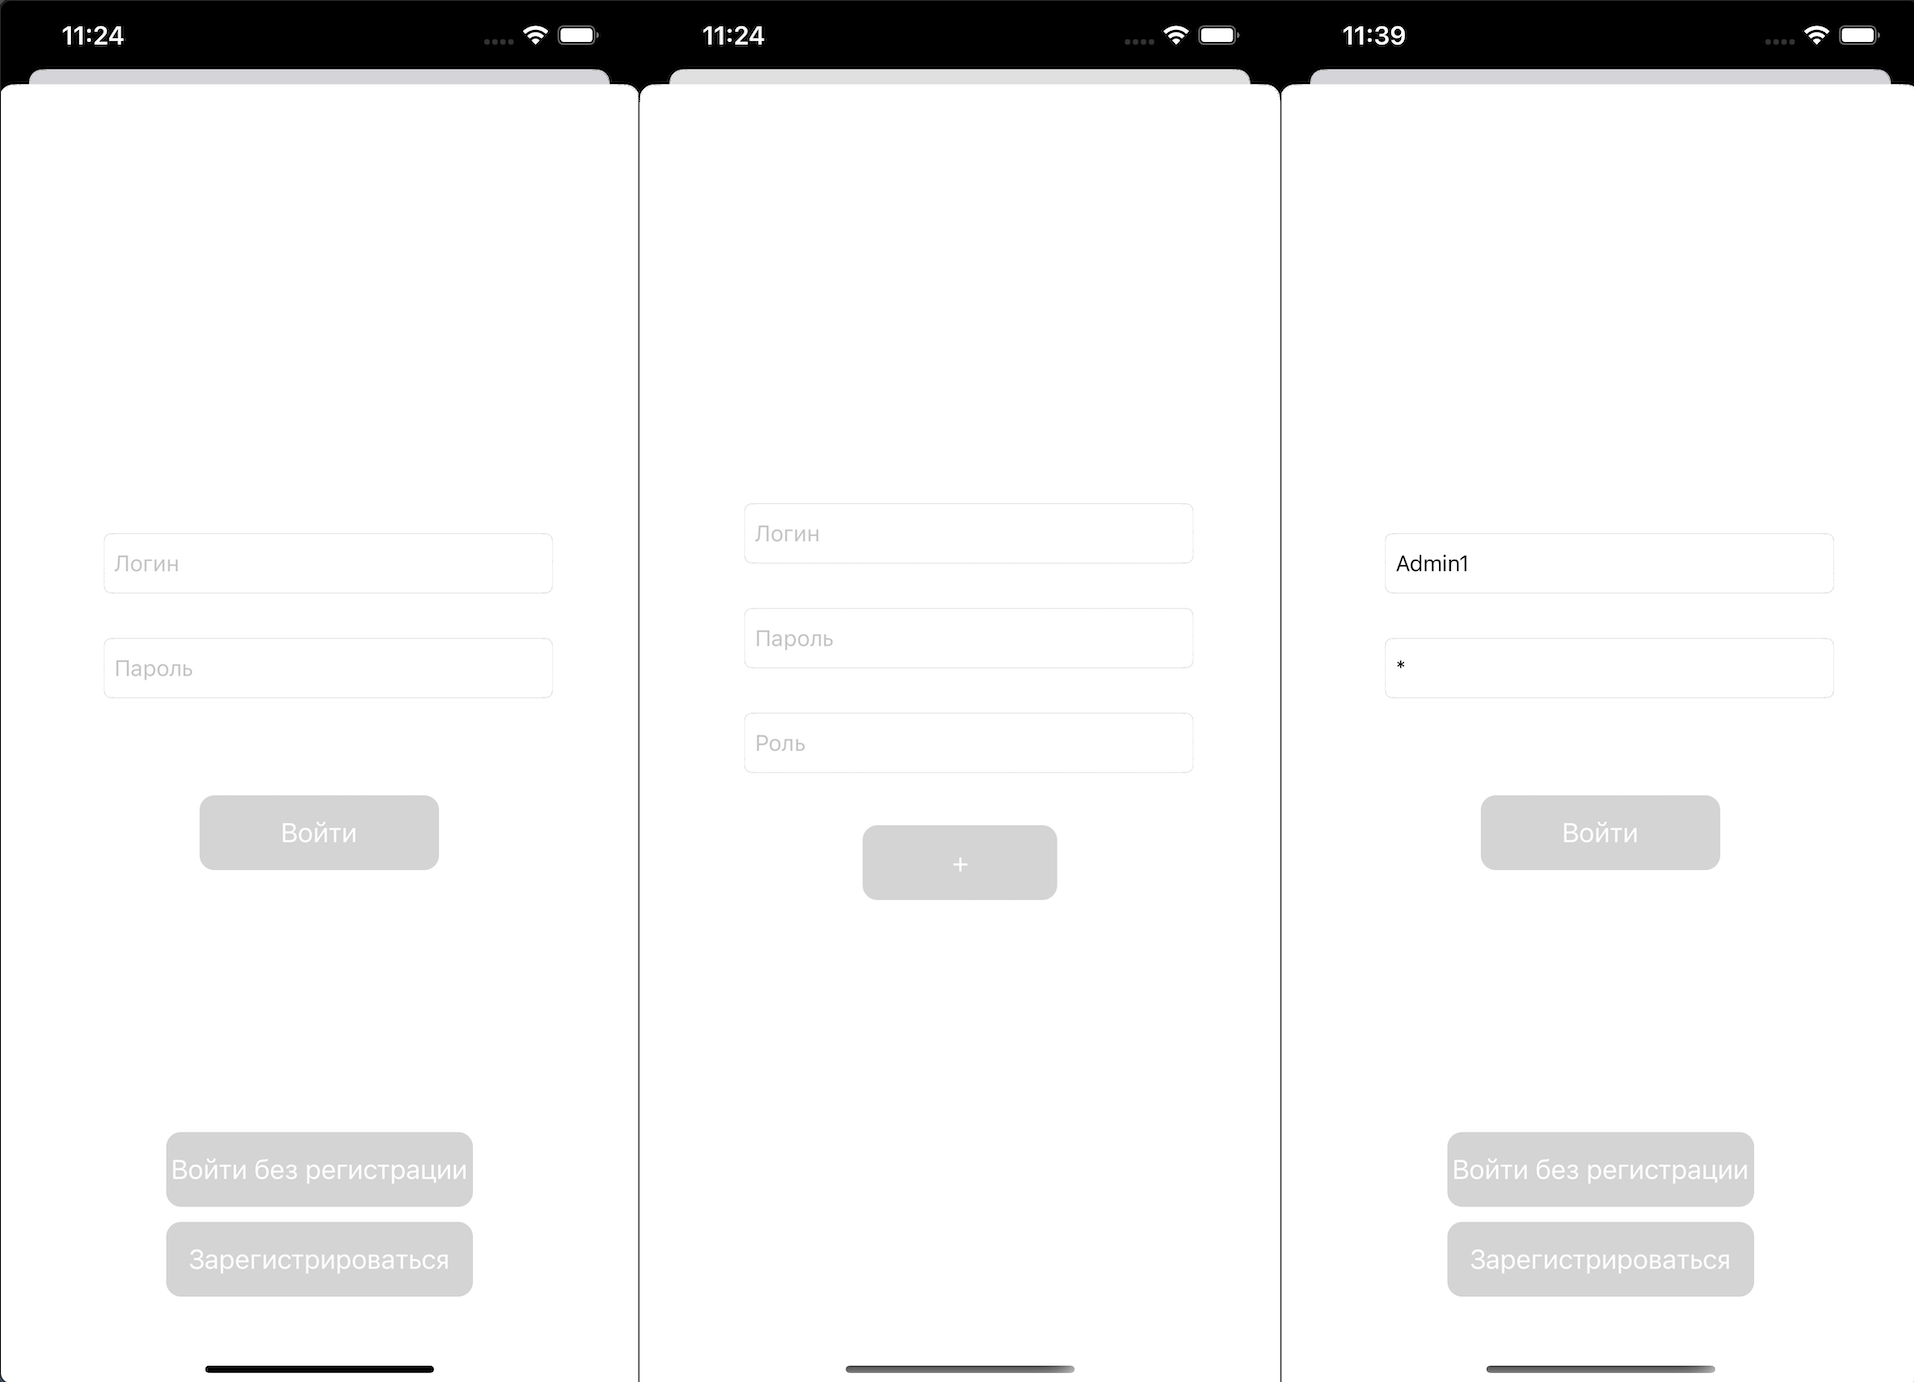
\includegraphics[scale=0.41]{img/gui/gui1}}
	\caption{Экраны персонализации}
	\label{fig:gui1}
\end{figure}

\begin{figure}[ht!]
	\centering{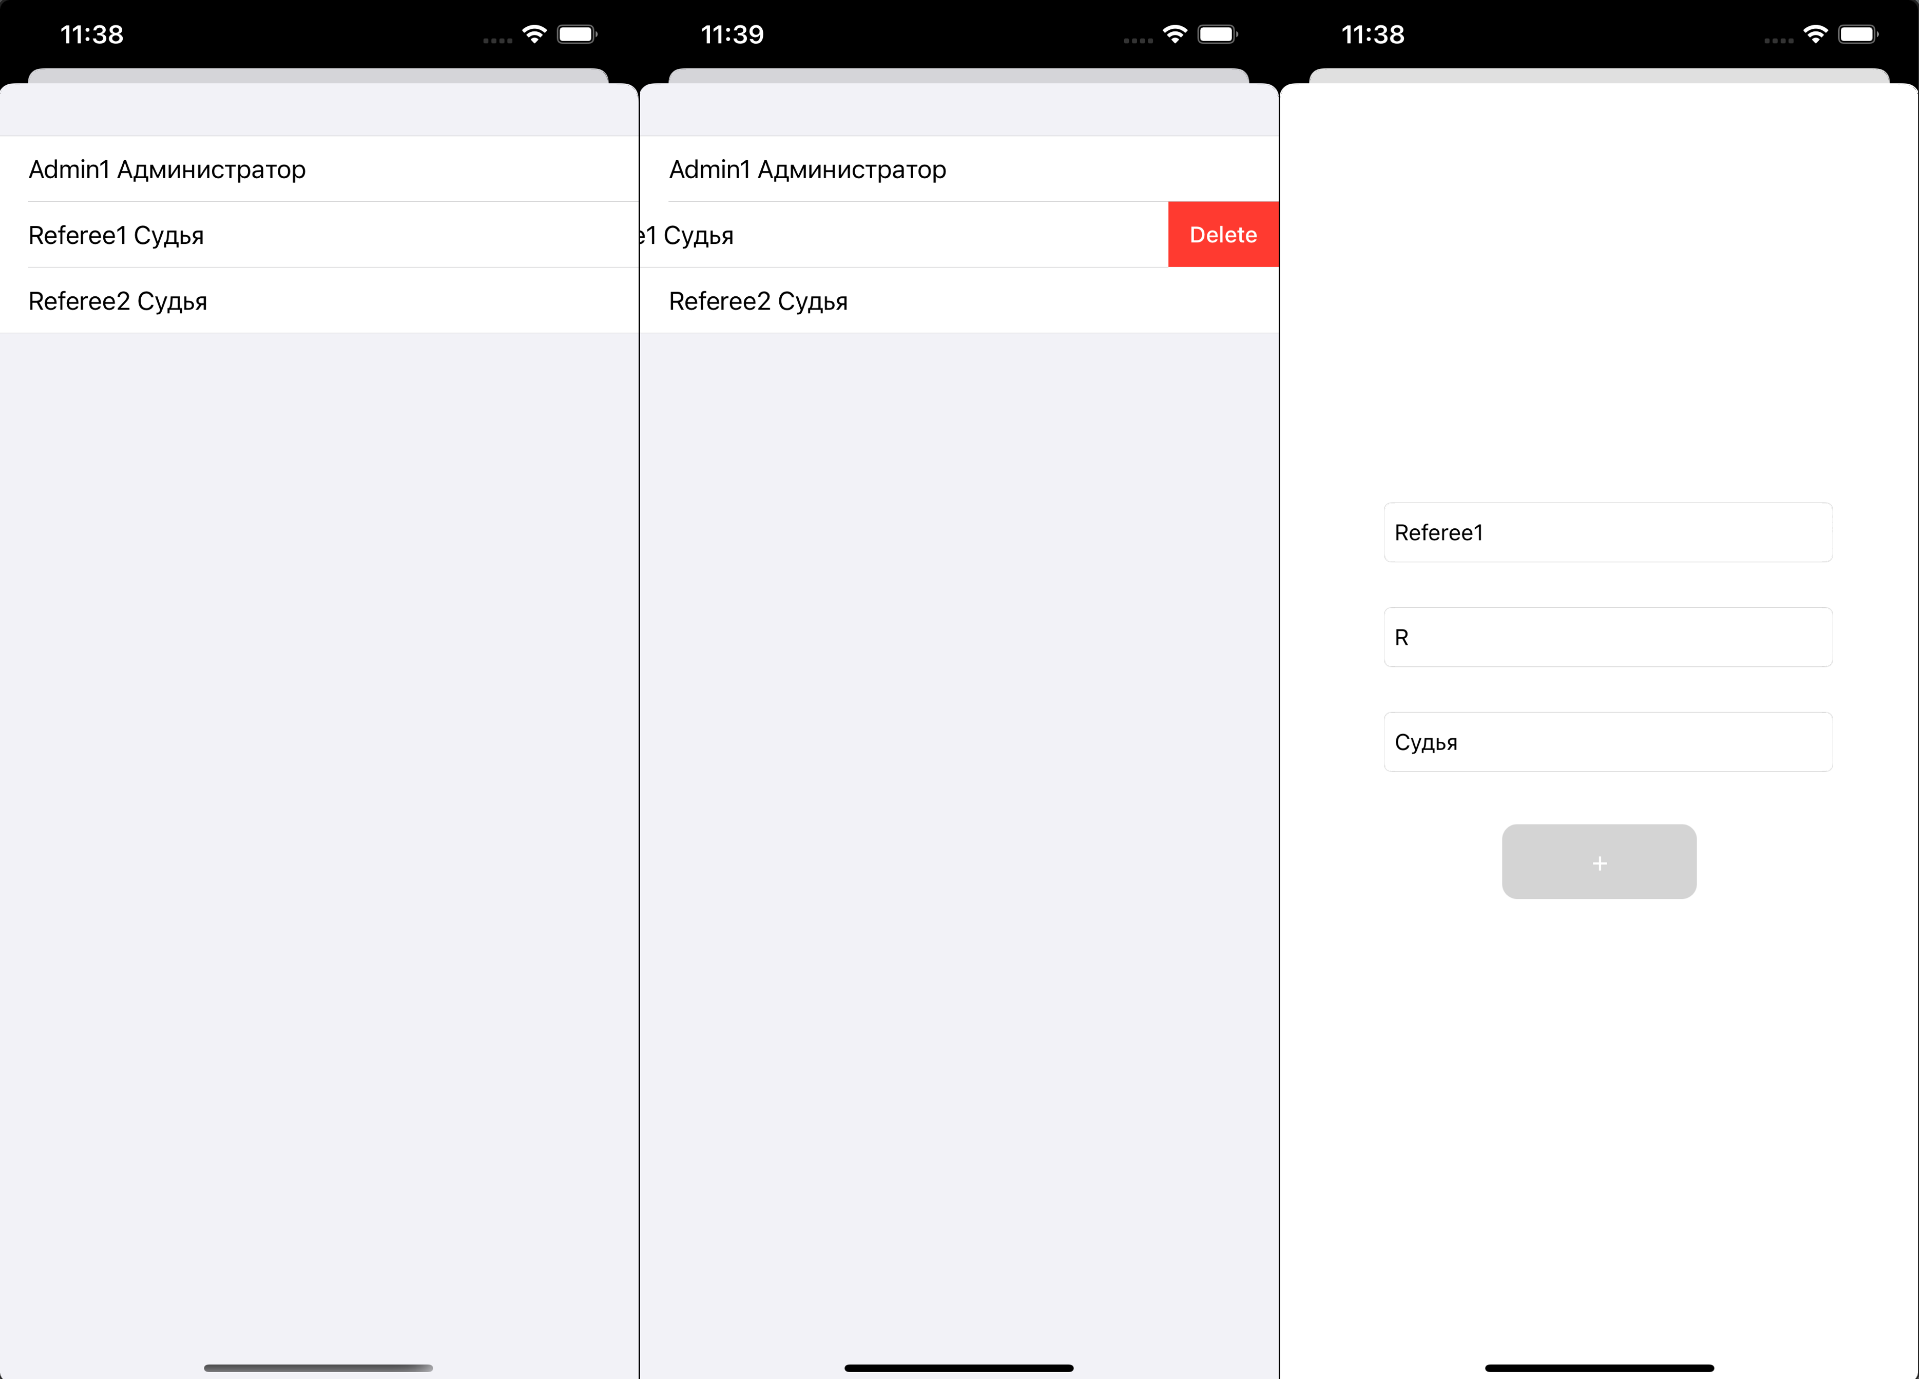
\includegraphics[scale=0.41]{img/gui/gui2}}
	\caption{Экраны доступа к данным об авторизованных пользователях системы (для администратора)}
	\label{fig:gui2}
\end{figure}

\begin{figure}[ht!]
	\centering{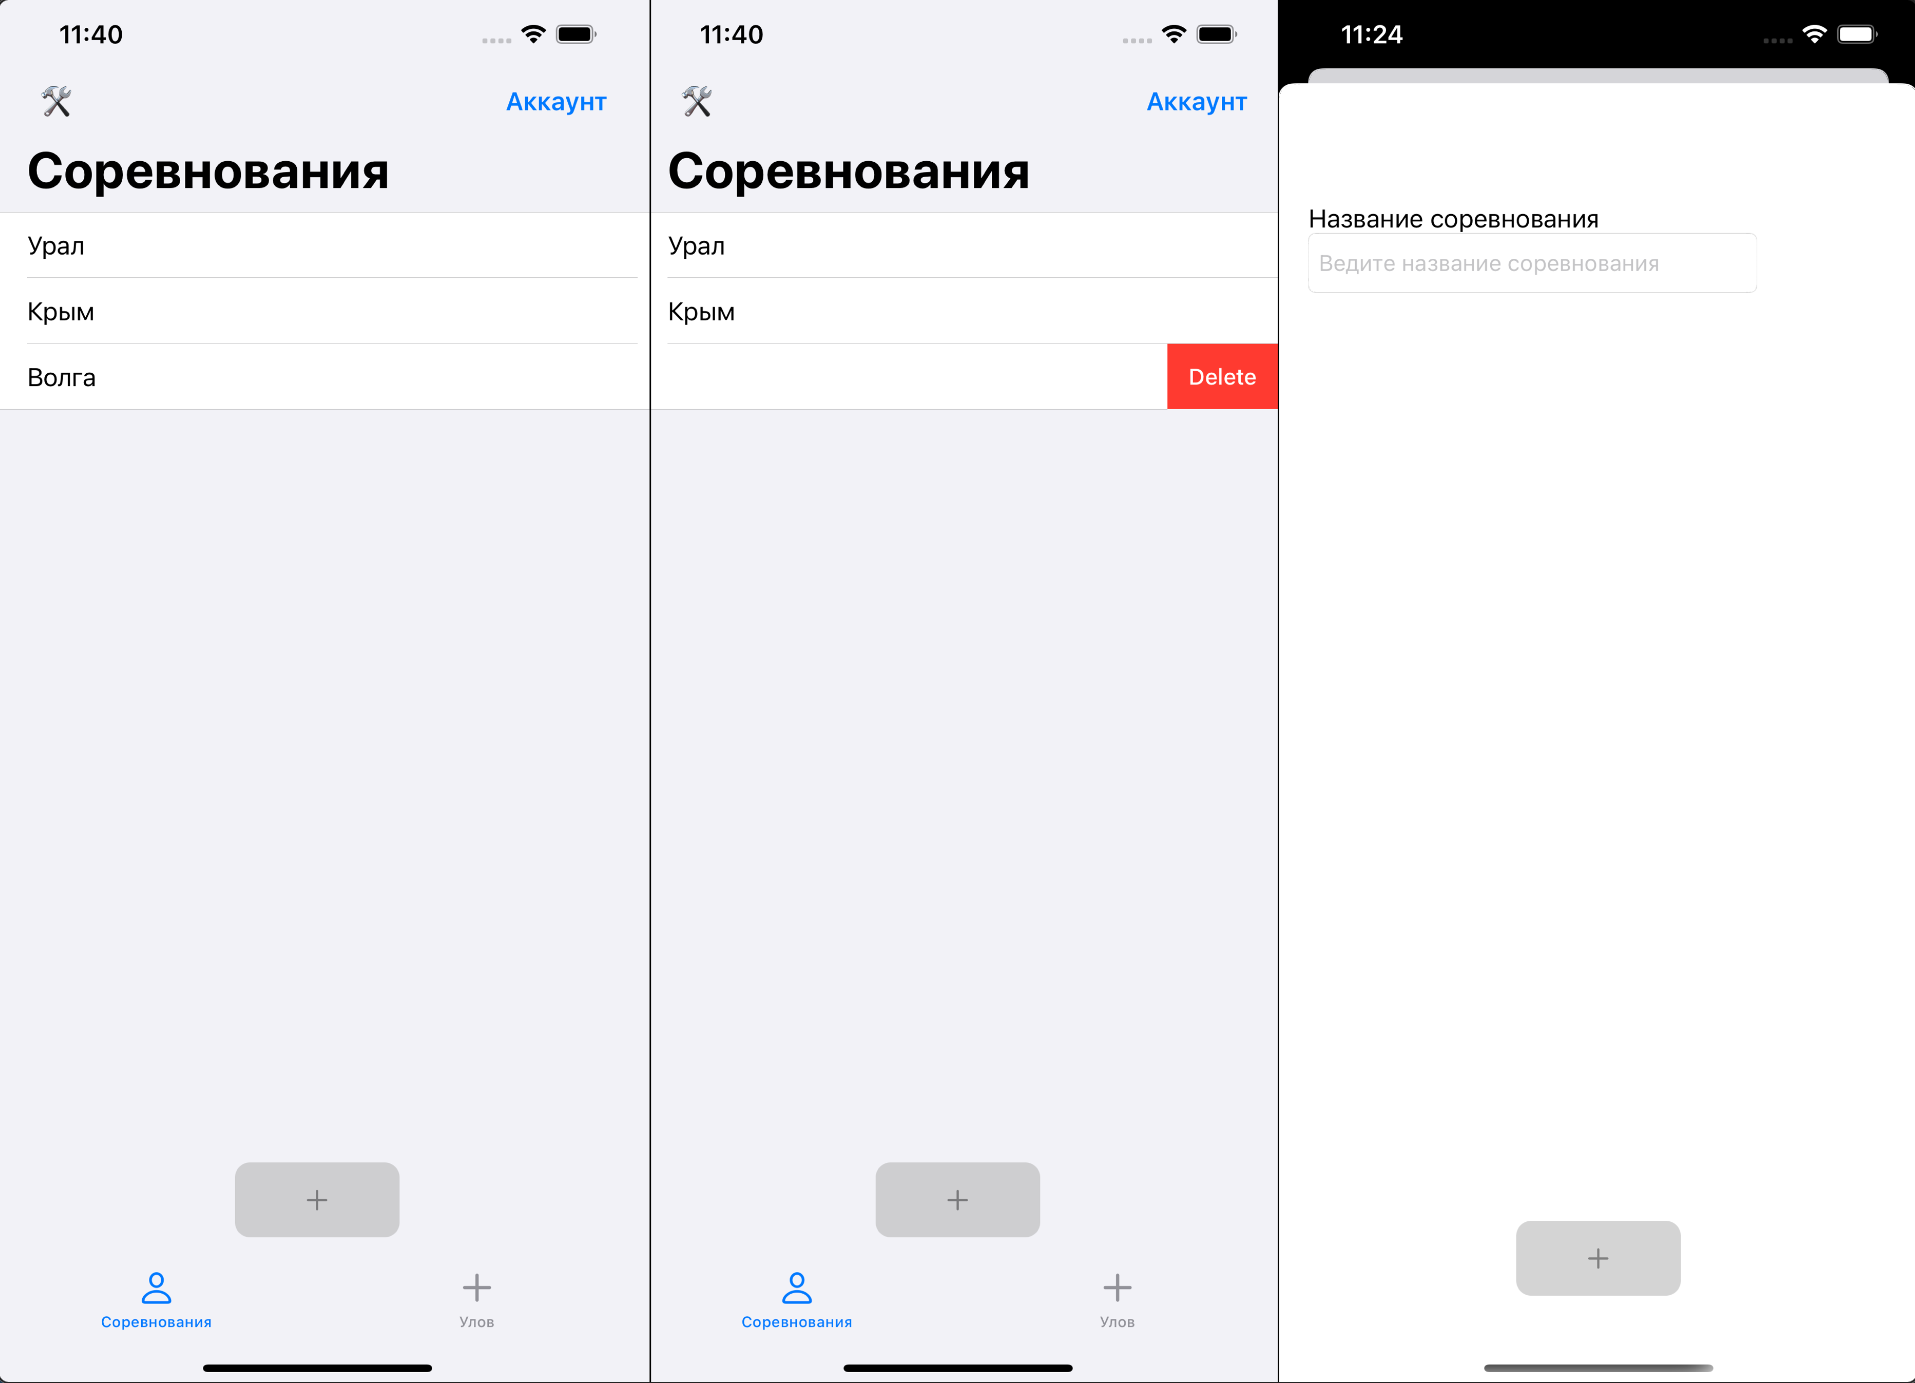
\includegraphics[scale=0.45]{img/gui/gui3}}
	\caption{Экраны формирования соревнований}
	\label{fig:gui3}
\end{figure}

\begin{figure}[ht!]
	\centering{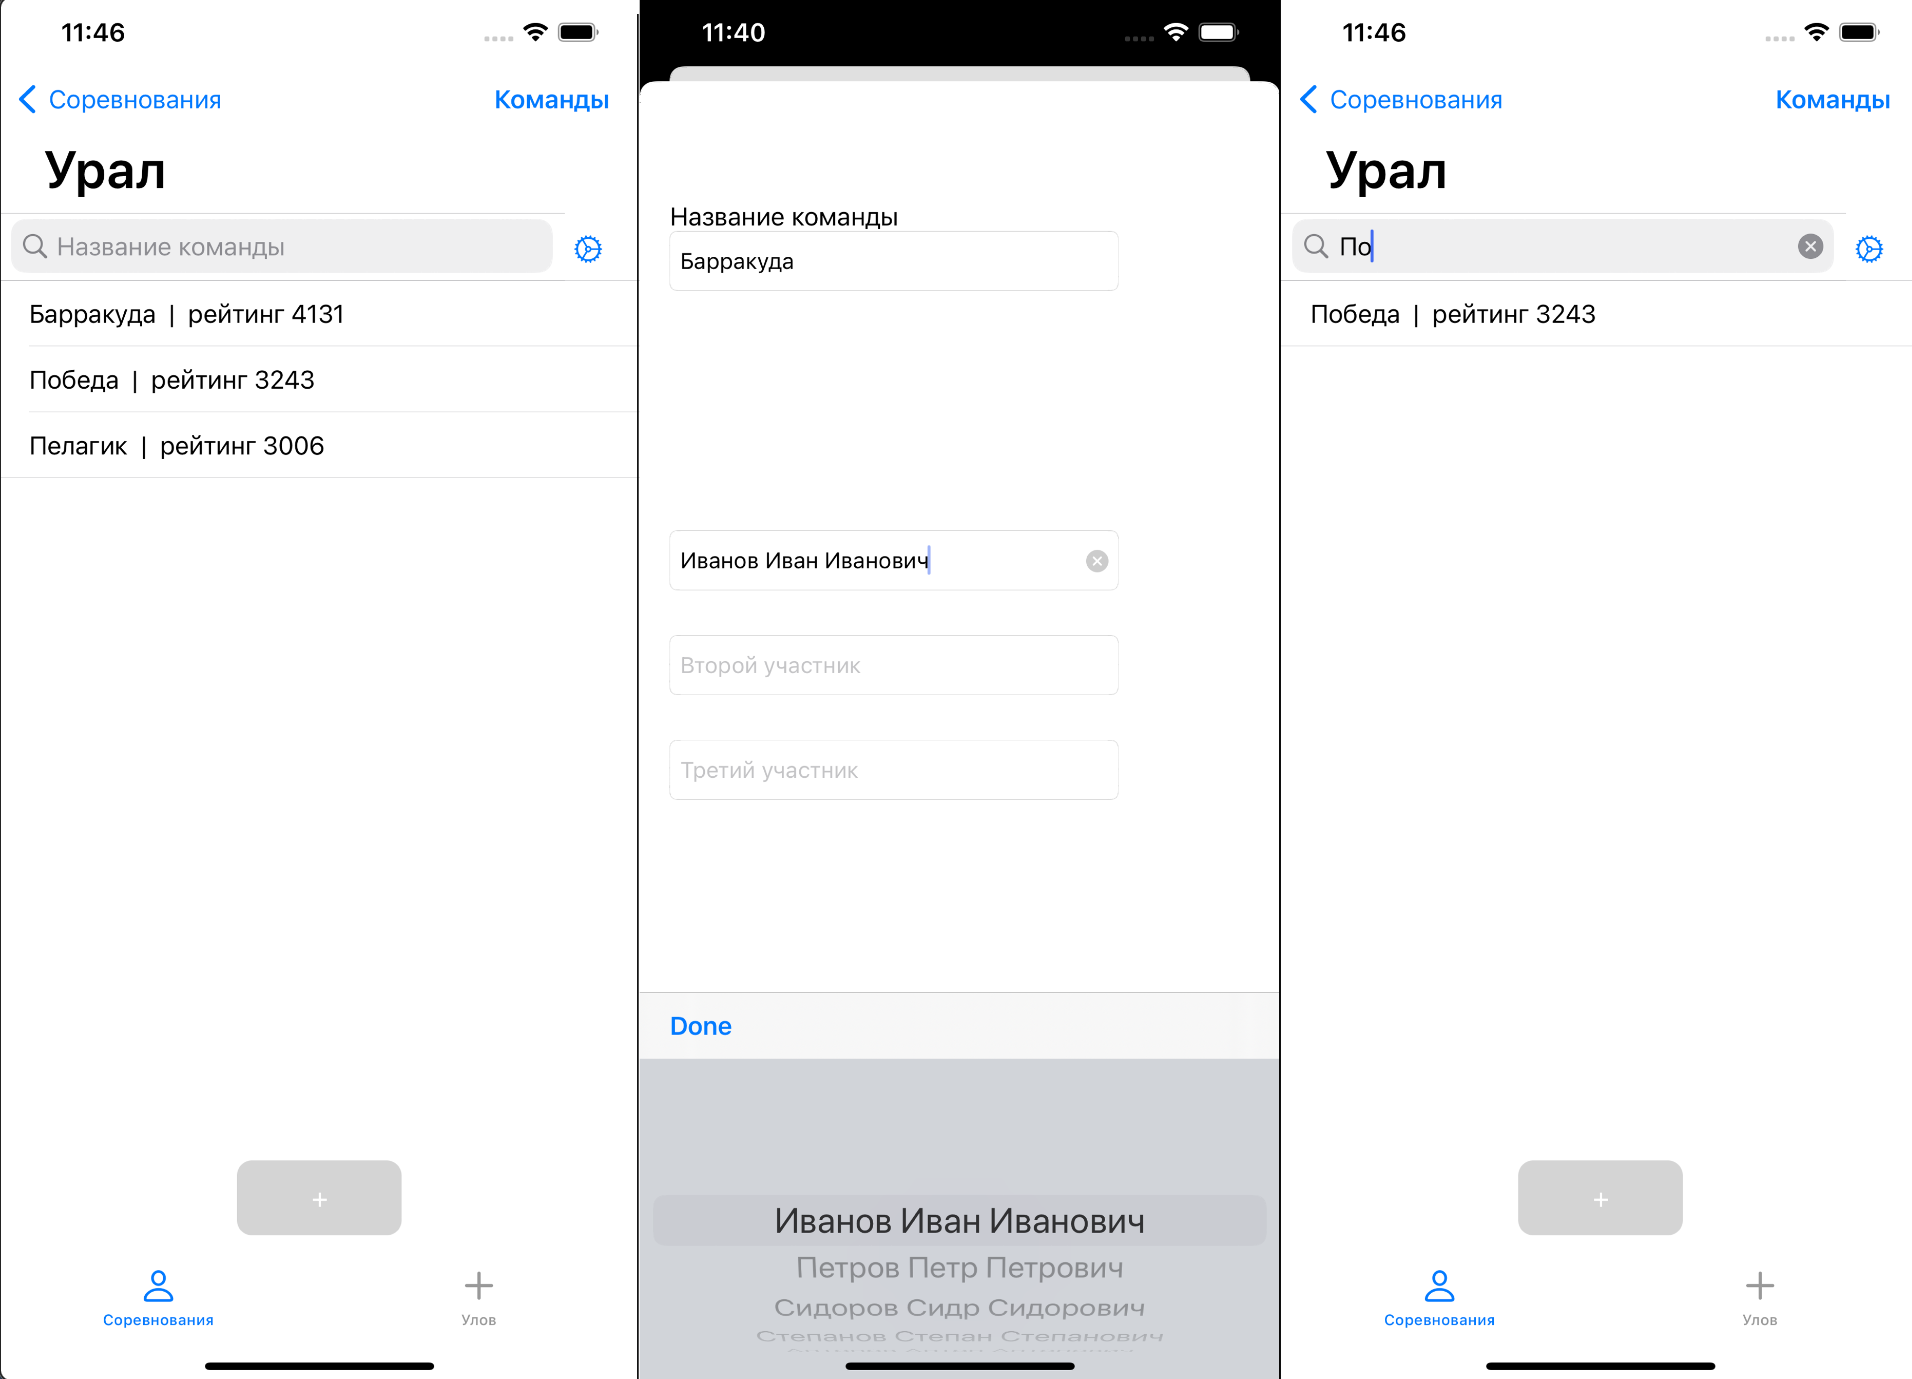
\includegraphics[scale=0.45]{img/gui/gui4}}
	\caption{Экраны формирования команд}
	\label{fig:gui4}
\end{figure}

\begin{figure}[ht!]
	\centering{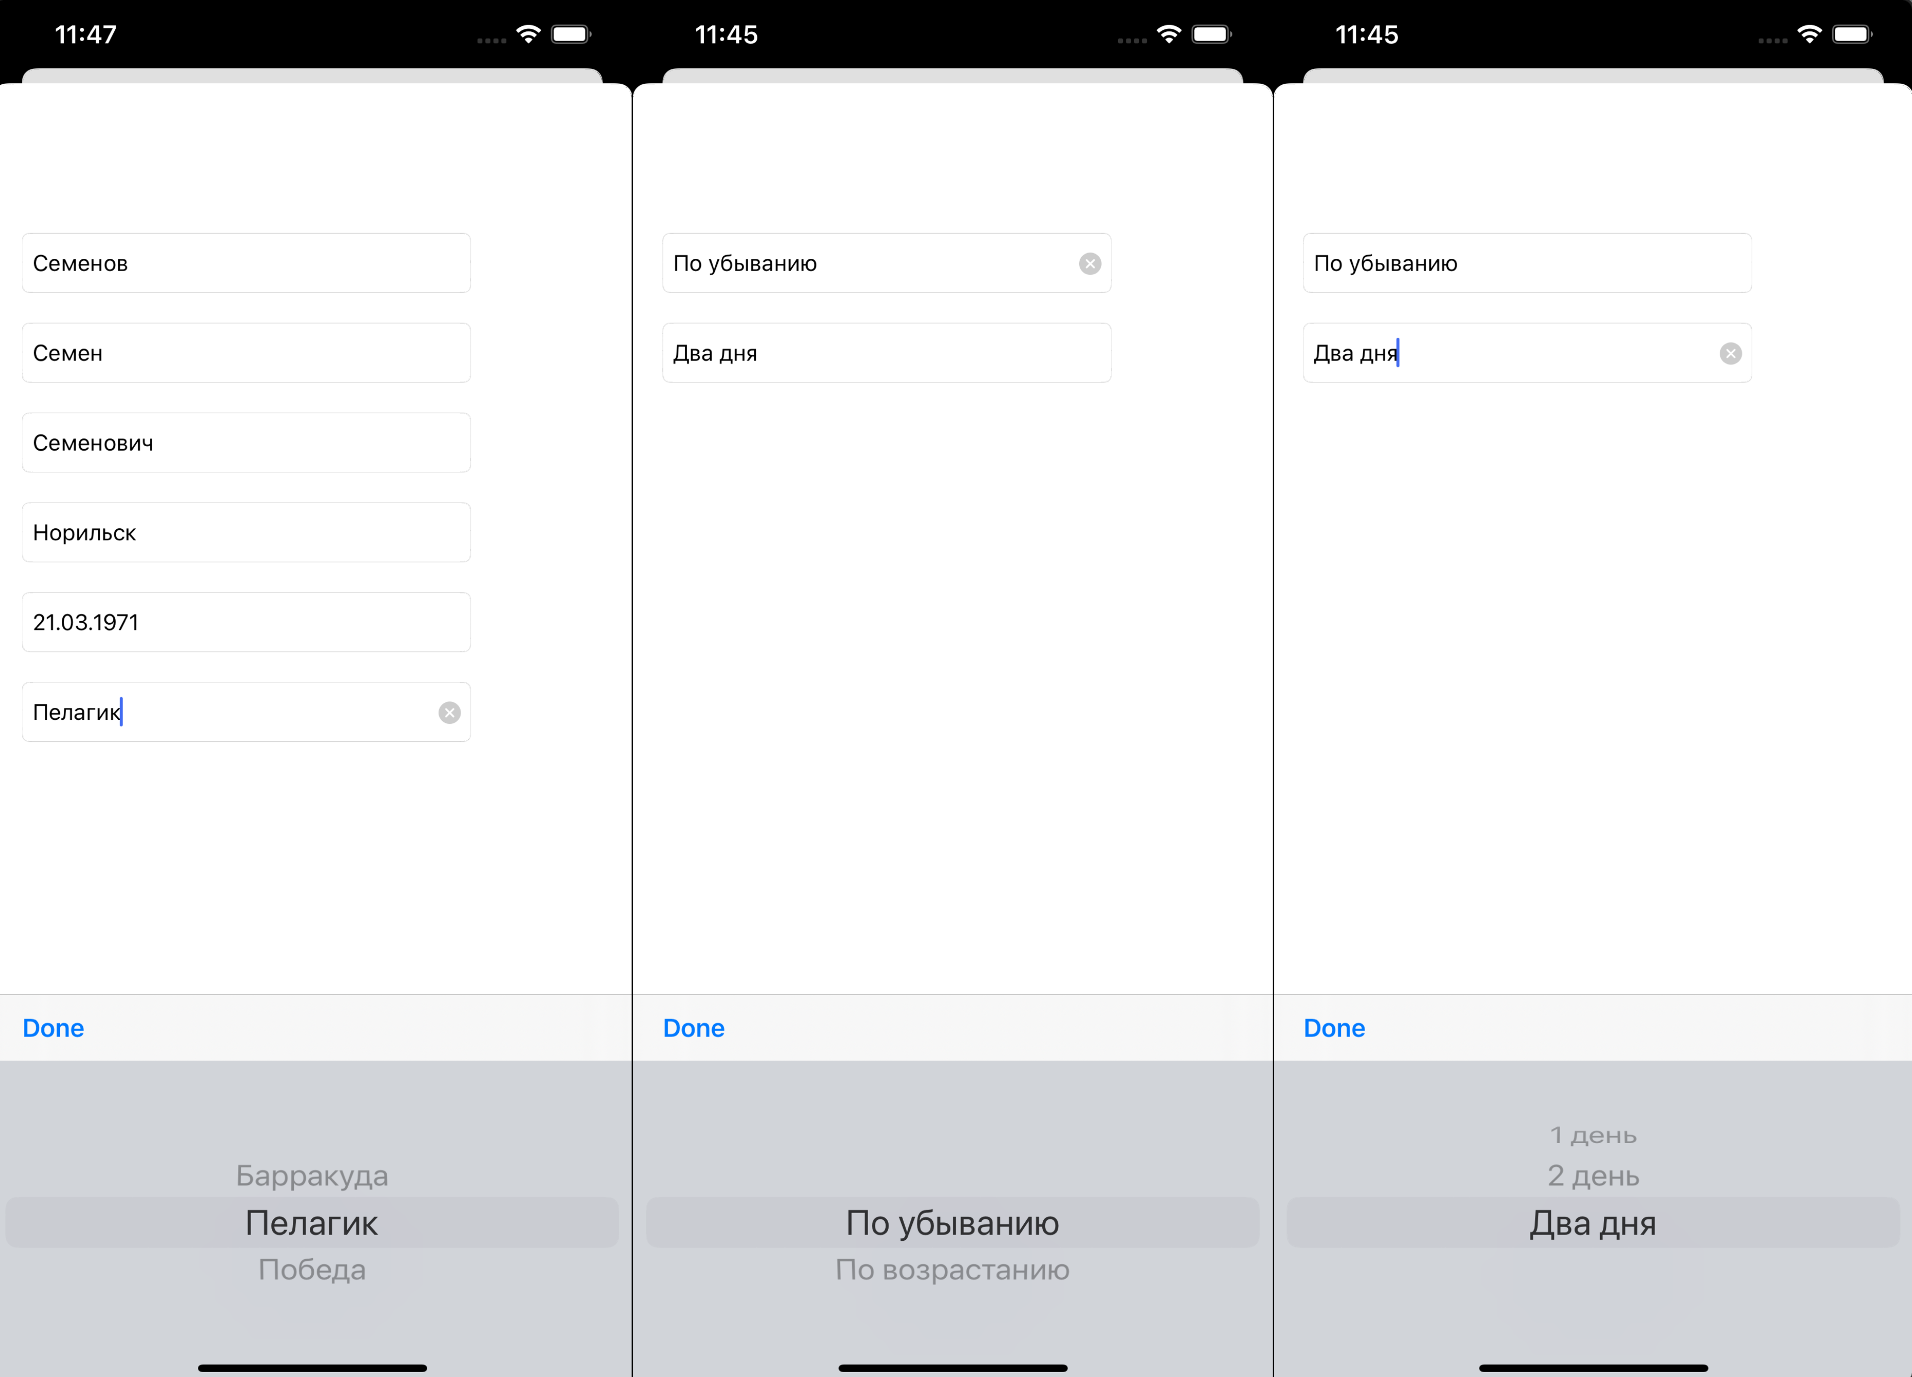
\includegraphics[scale=0.45]{img/gui/gui5}}
	\caption{Экраны создания участника, настройки параметров сортировки}
	\label{fig:gui5}
\end{figure}

\begin{figure}[ht!]
	\centering{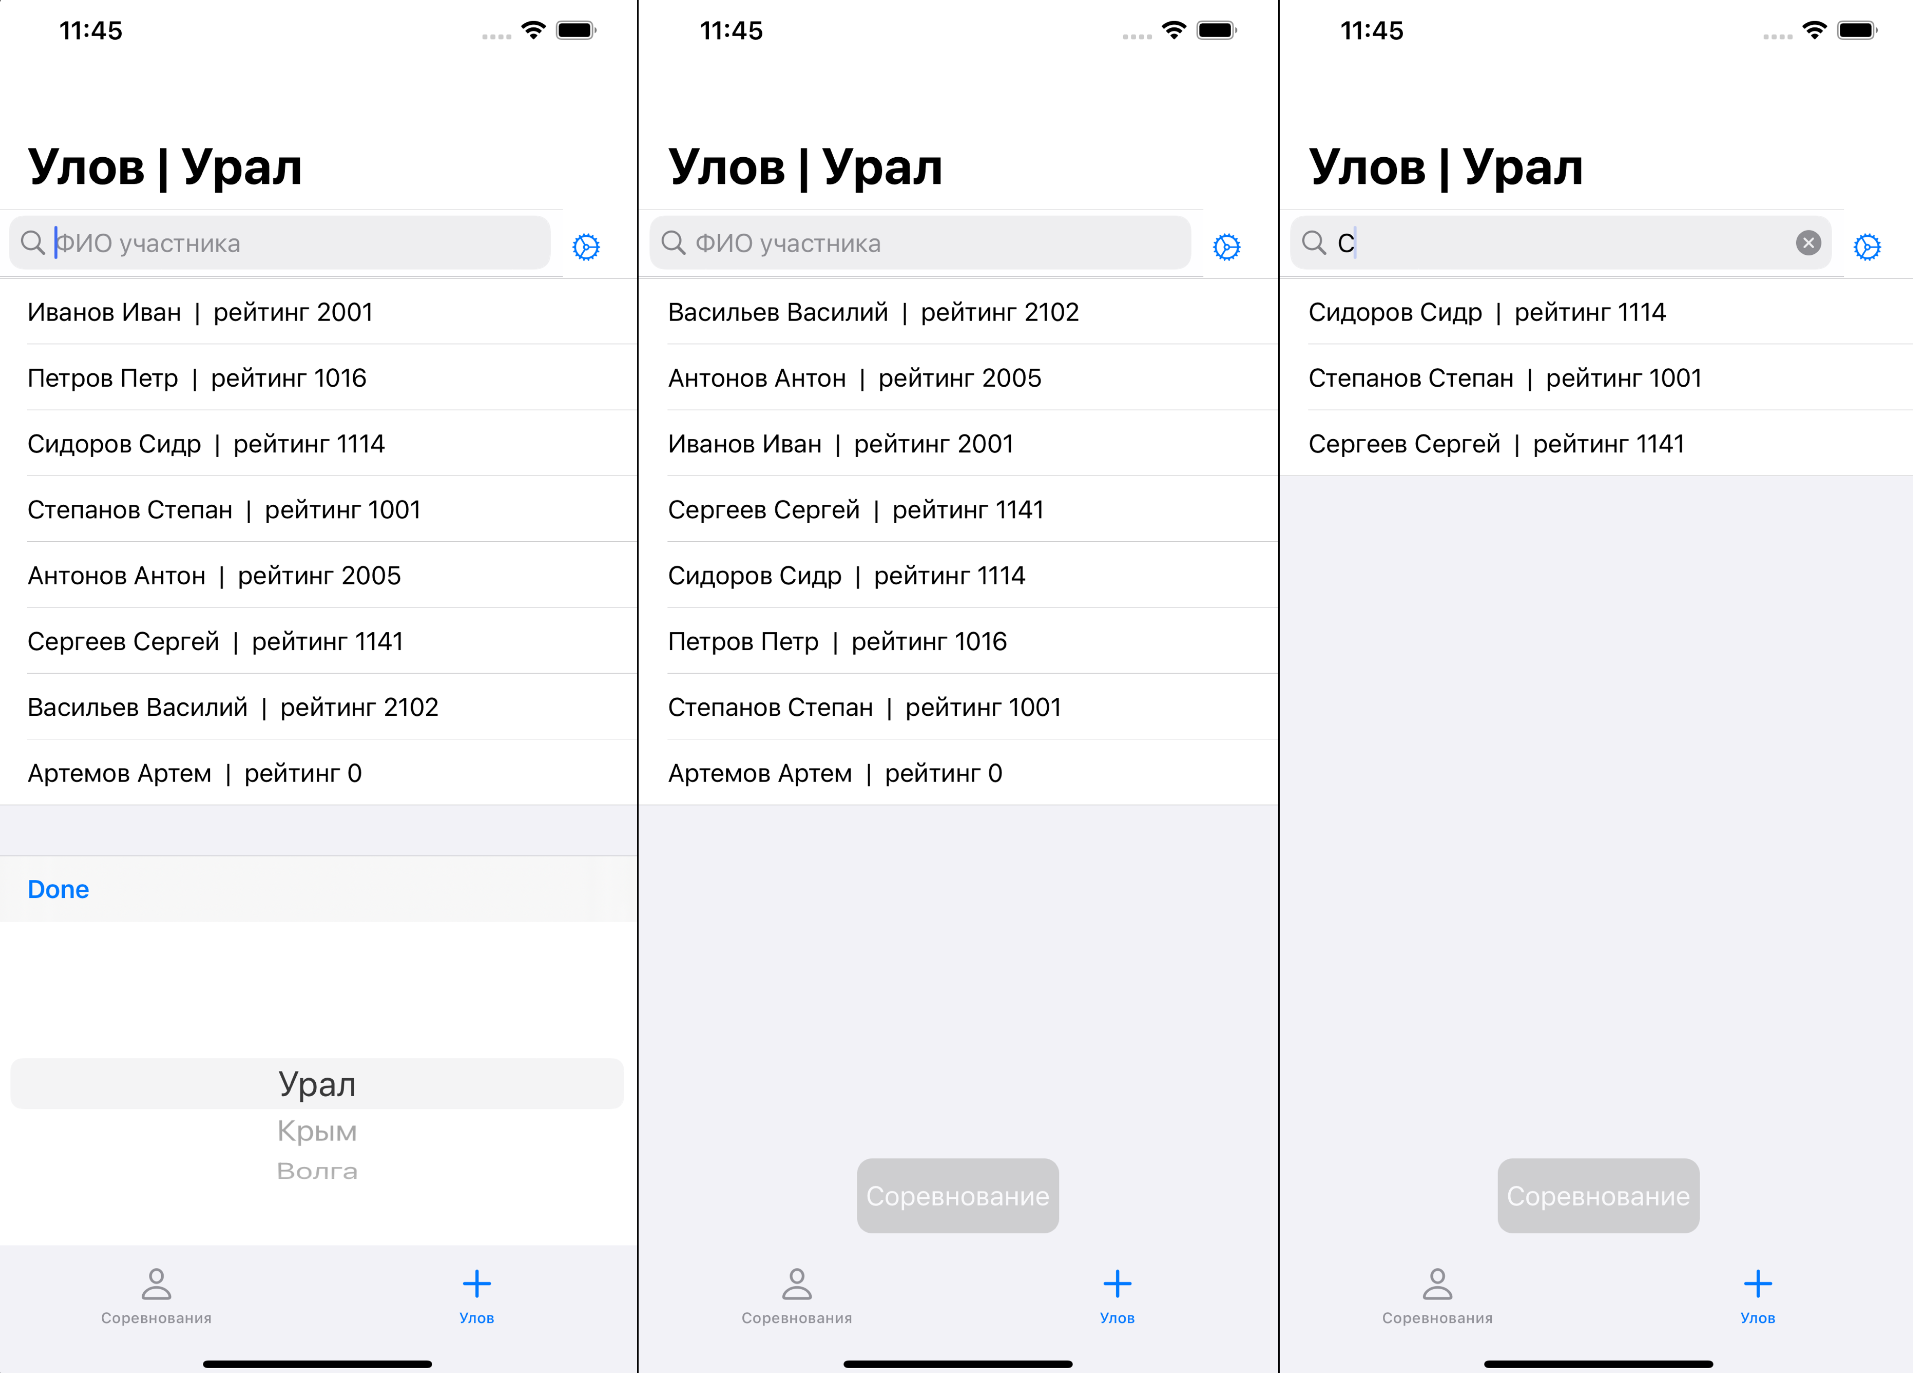
\includegraphics[scale=0.45]{img/gui/gui6}}
	\caption{Экраны формирования улова}
	\label{fig:gui6}
\end{figure}

\begin{figure}[ht!]
	\centering{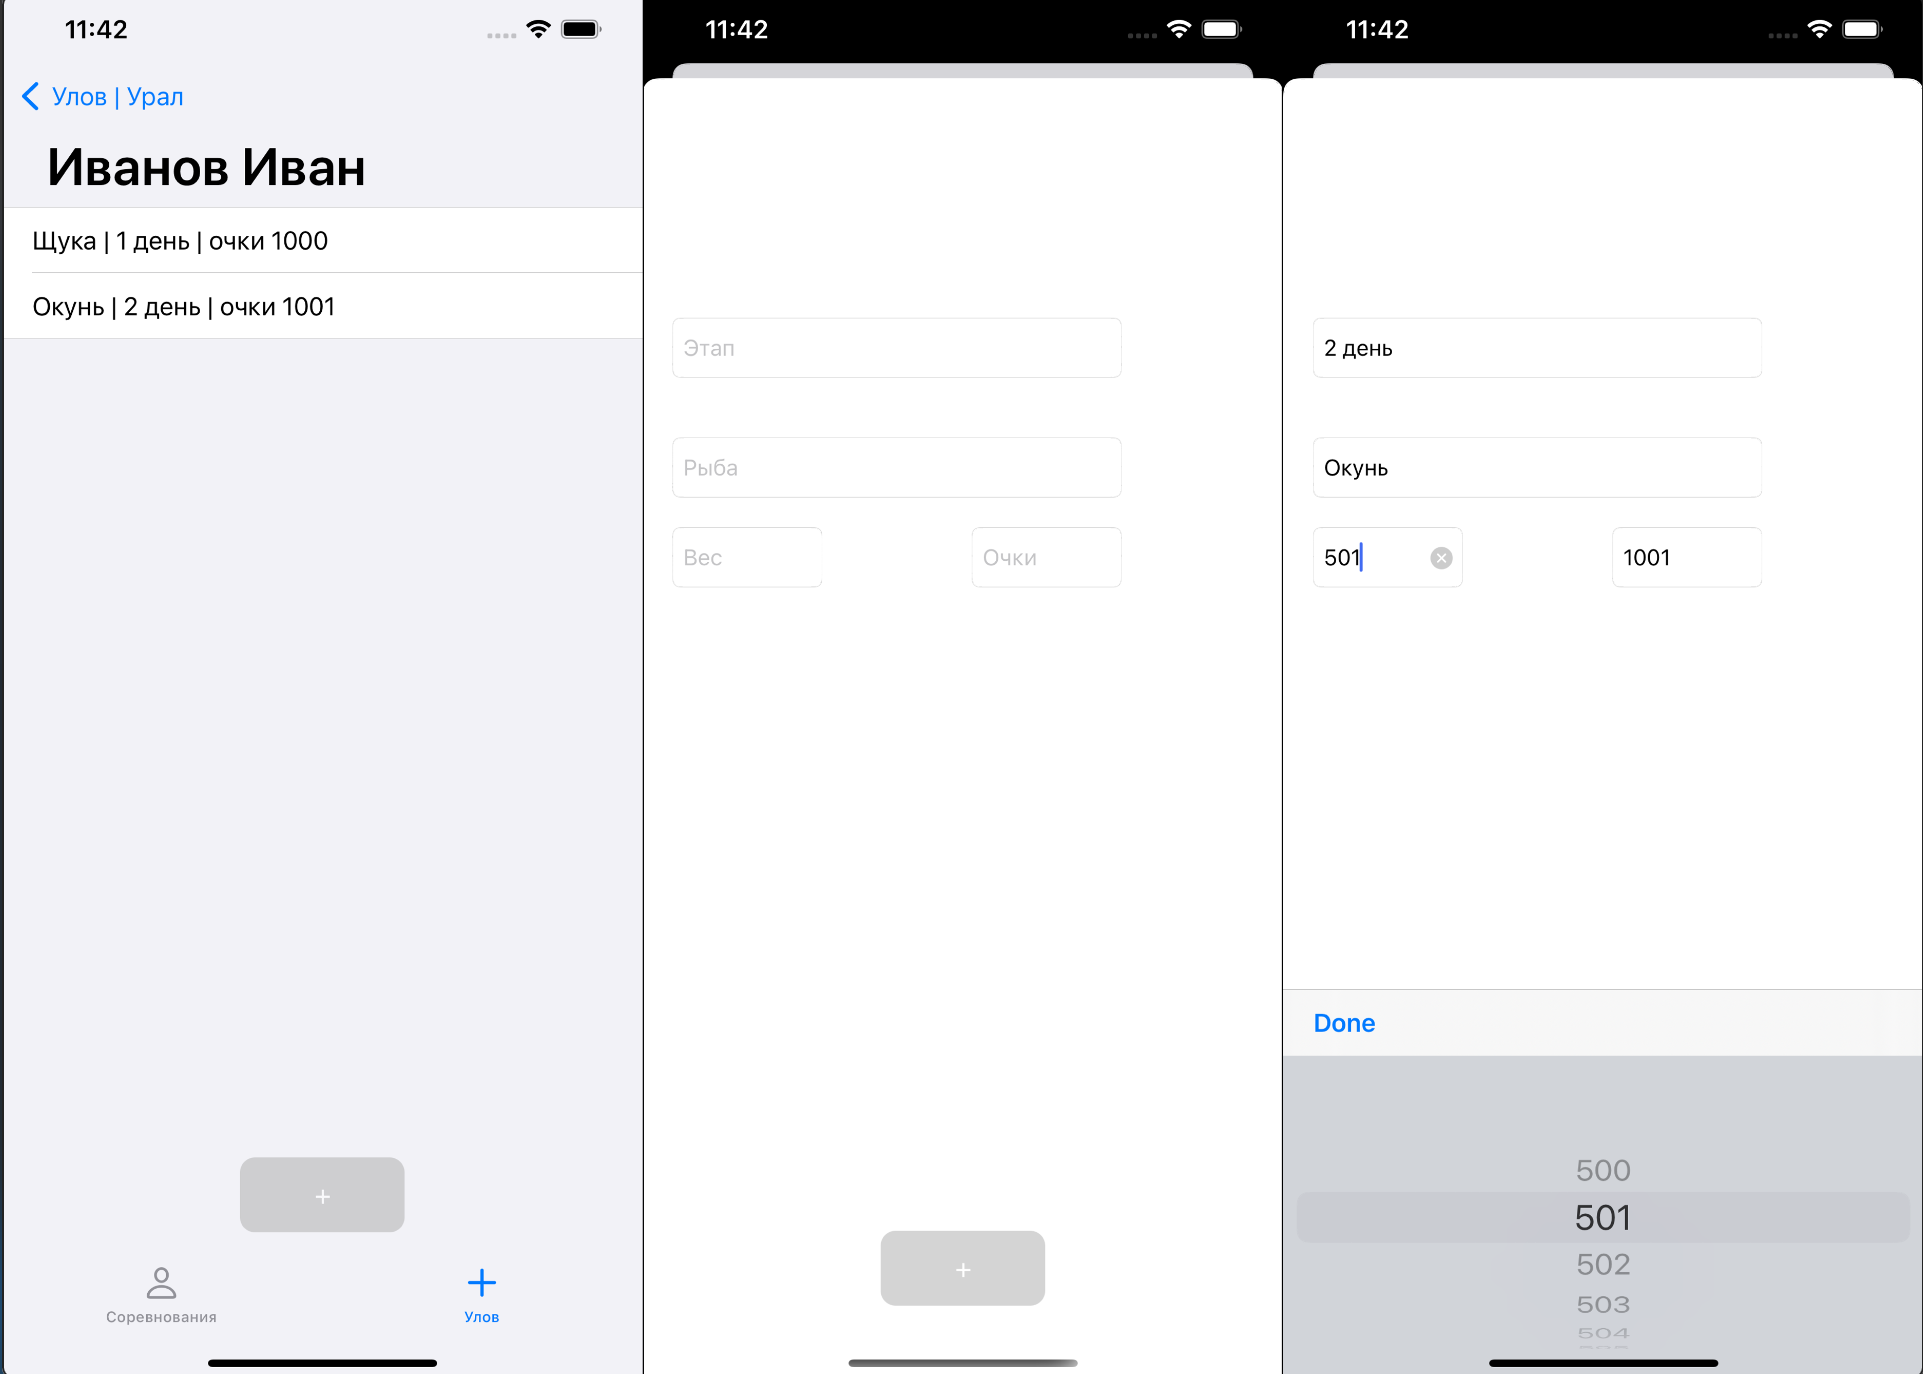
\includegraphics[scale=0.45]{img/gui/gui7}}
	\caption{Экраны формирования улова}
	\label{fig:gui7}
\end{figure}
